% Drawing 146/02-1 -- folder 146, batch 02, archive page 21 (PDF page 22).
% Transcription: Un grand cercle, sur lequel sont marqués et nommés des points : en haut $\widetilde{R}^\omega_k$, $\widetilde{R}_k$, $\widetilde{R}^{\omega'}_k$, puis en tournant $\widetilde{Q}^{\omega'}_j$, $-\widetilde{R}_i$ et ses deux voisins, $\widetilde{Q}^\omega_k$, $\widetilde{R}_j$ et ses deux voisins, $\widetilde{Q}^{\omega'}_i$, en bas $-\widetilde{R}^{\omega'}_k$, $-\widetilde{R}_k$, $-\widetilde{R}^\omega_k$, puis $\widetilde{Q}^\omega_j$, $\widetilde{R}_i$ et ses voisins, $\widetilde{Q}^{\omega'}_k$, $-\widetilde{R}_j$ et ses voisins, $\widetilde{Q}^\omega_i$. Chacun des six points $\pm\widetilde{R}$ est entouré d'un petit demi-cercle ; deux triangles inscrits forment une étoile à six branches, et quelques traits au crayon partent du centre et vers l'extérieur.
% Kind: circle with marked points (hexagonal symmetry). Method 2 (schematic redraw from the facsimile). Status: ok.
% Notes: Circle with 18 named points: six triples ±R~ (R~^omega, R~, R~^omega') each with a small half-circle round the middle point, and six Q~ between them; the two inscribed triangles join R~_k, R~_i, R~_j and -R~_k, -R~_i, -R~_j (pencil). Pencil strokes from the centre and towards the outside drawn as seen; the far end of the long stroke at the bottom right (a dot) is kept. Labels placed after the transcription.
% Coordinates: 1 unit = 1 mm = 1/100 of the crop width (bbox in page fractions: [0.12, 0.065, 0.62, 0.48]).
% Redrawn by Claude (claude-opus-5-5), issue #73 pilot, 2026-11-07; not checked by a human; not compiled (no TeX in the session).
% Rights: reproduces part of the work -- behind RENDER_TRANSCRIPTS, never published by itself.
\documentclass[tikz,border=3pt]{standalone}
\usepackage{amsmath,amssymb}
\usetikzlibrary{patterns,arrows.meta}
\tikzset{pencil/.style={black!45}, struck/.style={black!35}, mark/.style={circle,draw,inner sep=1.3pt}, pt/.style={circle,fill,inner sep=0.9pt}, opt/.style={circle,draw,fill=white,inner sep=1.1pt}}
\begin{document}
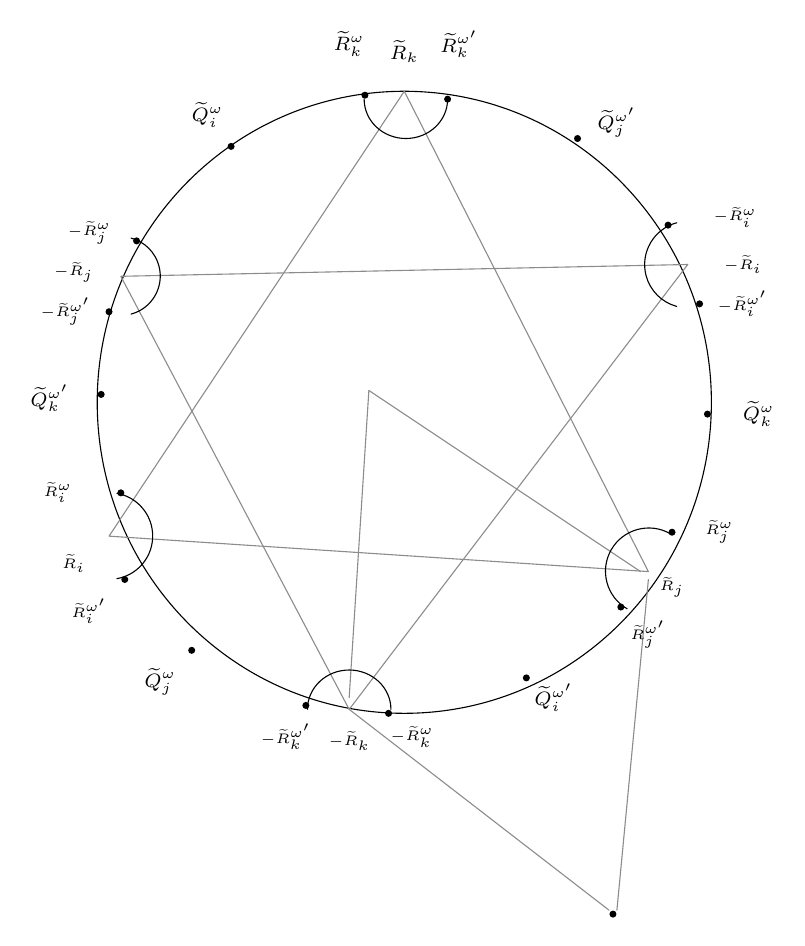
\begin{tikzpicture}[x=1mm,y=1mm,line cap=round,line join=round,font=\scriptsize]
\draw (52,-50.5) ellipse[x radius=39, y radius=39.5];
\draw[pencil] (52,-11) -- (14.5,-67.5) -- (83,-72) -- cycle;
\draw[pencil] (45,-89.5) -- (16,-34.5) -- (88,-33) -- cycle;
\draw[pencil] (47.5,-49) -- (82,-72);
\draw[pencil] (47.5,-49) -- (45,-88);
\draw[pencil] (45,-89.5) -- (78,-115);
\draw[pencil] (83,-73) -- (79,-115);
\node[pt] at (78.5,-115.5) {};
\node[pt] at (47,-11.5) {};
\node[pt] at (57.5,-12) {};
\draw (46.9,-12) arc[start angle=180, end angle=360, x radius=5.3, y radius=5];
\node[pt] at (85.5,-28) {};
\node[pt] at (89.5,-38) {};
\draw (86.6,-27.7) arc[start angle=105, end angle=255, x radius=5.5, y radius=5.5];
\node[pt] at (86,-67) {};
\node[pt] at (79.5,-76.5) {};
\draw (85.8,-67.2) arc[start angle=60, end angle=240, x radius=5.5, y radius=5.5];
\node[pt] at (39.5,-89) {};
\node[pt] at (50,-90) {};
\draw (50.3,-89.5) arc[start angle=0, end angle=180, x radius=5.3, y radius=5];
\node[pt] at (16,-62) {};
\node[pt] at (16.5,-73) {};
\draw (15.5,-72.9) arc[start angle=-80, end angle=80, x radius=5.5, y radius=5.5];
\node[pt] at (18,-30) {};
\node[pt] at (14.5,-39) {};
\draw (17.3,-39.3) arc[start angle=-75, end angle=75, x radius=5, y radius=5];
\node[pt] at (30,-18) {};
\node[pt] at (74,-17) {};
\node[pt] at (90.5,-52) {};
\node[pt] at (67.5,-85.5) {};
\node[pt] at (25,-82) {};
\node[pt] at (13.5,-49.5) {};
\node[inner sep=1pt] at (45,-5) {\scriptsize $\widetilde{R}^\omega_k$};
\node[inner sep=1pt] at (52,-6) {\scriptsize $\widetilde{R}_k$};
\node[inner sep=1pt] at (59,-5) {\scriptsize $\widetilde{R}^{\omega'}_k$};
\node[inner sep=1pt] at (79,-15) {\scriptsize $\widetilde{Q}^{\omega'}_j$};
\node[inner sep=1pt] at (94,-27) {\tiny $-\widetilde{R}^{\omega}_i$};
\node[inner sep=1pt] at (95,-33) {\tiny $-\widetilde{R}_i$};
\node[inner sep=1pt] at (95,-38) {\tiny $-\widetilde{R}^{\omega'}_i$};
\node[inner sep=1pt] at (97,-52) {\scriptsize $\widetilde{Q}^\omega_k$};
\node[inner sep=1pt] at (92,-67) {\tiny $\widetilde{R}^{\omega}_j$};
\node[inner sep=1pt] at (86,-74) {\tiny $\widetilde{R}_j$};
\node[inner sep=1pt] at (83,-80) {\tiny $\widetilde{R}^{\omega'}_j$};
\node[inner sep=1pt] at (71,-88) {\scriptsize $\widetilde{Q}^{\omega'}_i$};
\node[inner sep=1pt] at (37,-93) {\tiny $-\widetilde{R}^{\omega'}_k$};
\node[inner sep=1pt] at (45,-93.5) {\tiny $-\widetilde{R}_k$};
\node[inner sep=1pt] at (53,-93) {\tiny $-\widetilde{R}^\omega_k$};
\node[inner sep=1pt] at (21,-86) {\scriptsize $\widetilde{Q}^\omega_j$};
\node[inner sep=1pt] at (8,-62) {\tiny $\widetilde{R}^{\omega}_i$};
\node[inner sep=1pt] at (10,-71) {\tiny $\widetilde{R}_i$};
\node[inner sep=1pt] at (12,-77) {\tiny $\widetilde{R}^{\omega'}_i$};
\node[inner sep=1pt] at (7,-50) {\scriptsize $\widetilde{Q}^{\omega'}_k$};
\node[inner sep=1pt] at (12,-29) {\tiny $-\widetilde{R}^{\omega}_j$};
\node[inner sep=1pt] at (10,-34) {\tiny $-\widetilde{R}_j$};
\node[inner sep=1pt] at (9,-39) {\tiny $-\widetilde{R}^{\omega'}_j$};
\node[inner sep=1pt] at (27,-14) {\scriptsize $\widetilde{Q}^\omega_i$};
\end{tikzpicture}
\end{document}
